
\documentclass[11pt,a4paper]{article}

\usepackage{graphicx} % Required for the inclusion of images
\usepackage[utf8]{inputenc}
%\usepackage{natbib} % Required to change bibliography style to APA
\usepackage{amsmath} % Required for some math elements 
\usepackage[spanish]{babel} 
%\usepackage{fontspec}
\usepackage{lineno,hyperref}
\usepackage{upgreek}
\usepackage{gensymb}
\usepackage{textcomp}
\usepackage{amssymb}
\usepackage{textgreek}
\usepackage{float}
\usepackage{fancyhdr}
\usepackage{dirtytalk}
\allowdisplaybreaks
%\textwidth18cm
%\textheight22cm
%\topmargin0cm
%\oddsidemargin2cm
%\hypersetup{hidelinks}

\usepackage{multirow}

\hypersetup{
    colorlinks=true,
    linkcolor=blue,
    }
\graphicspath{{img}}
\setlength\parindent{0pt} % Removes all indentation from paragraphs

\renewcommand{\labelenumi}{\alph{enumi}.} % Make numbering in the enumerate environment by letter rather than number (e.g. section 6)

\renewcommand{\b}{\textbf}

\newsavebox{\mygraphic}
\sbox{\mygraphic}{
\includegraphics[height=1.5cm]{logoUNRN.jpg}}


\pagestyle{fancy}

\fancyhead{}

\headheight 16pt

\fancyhead[LO]{\setlength{\unitlength}{1in}
	\begin{picture}(0,0)
		\put(0,0){\usebox{\mygraphic}}
	\end{picture}
	\hspace{1cm}
}

\fancyhead[CO] {\hspace{1.5cm} Física I, Ingenierías ambiental, electrónica y telecomunicaciones}




%esto me pareció piola para enumerar los ejercicios
%lo saqué de acá: https://tex.stackexchange.com/questions/302948/numbered-exercises-as-sections
%%%%%%%%%%%%%%%%%%%%%%%%%%%%%%%%%%%%%%%%%5
\newcounter{eje}
\setcounter{eje}{0}
\newcounter{subeje}
\setcounter{subeje}{-1}
\renewcommand\thesubeje{\arabic{eje}\alph{subeje}}%
\newcommand \eje{%
  \par\noindent
  \ifnum\value{subeje}>-1
    \refstepcounter{subeje}%
    \llap{\thesubeje)\quad}%
  \else
    \refstepcounter{eje}%
    \llap{\theeje)\quad}%
  \fi
}
\begin{document}
\pagestyle{fancy}

\begin{center}
%%	\centering
	{\Large \textbf{Práctica 0}}

{Incertidumbre, unidades y vectores}
\end{center}



\subsection*{Preguntas}
Responda las siguientes preguntas, explicando con claridad sus razonamientos.
\eje ¿Qué fenómenos físicos podrían servir para definir un estándar de tiempo?.
\eje ¿Cuáles son las unidades de volumen?
\eje Explique las diferencias entre exactitud y precisión.
\eje ¿Puede encontrar dos vectores de distinta longitud y que su suma sea nula? ¿Qué restricciones de longitud son
necesarias para que tres vectores tengan resultante cero?
\eje Sean \b A y \b B dos vectores distintos de cero. Explique cuándo se anula el producto escalar y el producto vectorial entre
ellos.
\eje Sea \b A un vector cualquiera distinto de cero ¿Por qué \b A/A es un vector unitario y qué dirección tiene?
\eje De al menos tres ejemplos de magnitudes vectoriales y otros tres de magnitudes escalares.


\subsection*{Problemas}
\setcounter{eje}{0}

\eje Conversiones de unidades: Realice las siguientes conversiones de unidades según se indique.

a) 0.473 L a pulgadas cúbicas sabiendo que 1L=1000cm$^3$ y 1in=2.54cm

b) La densidad del plomo es 11.3 g/cm, exprese en kg/m$^3$ .

c) 327 in$^3$ a L y m$^3$

d) La velocidad de la luz en el vacío es c=300 10$^3$ km/s expresar esta cantidad en m/s, km/h y millas por minutos (mi/min)

\eje Calcule el tiempo en nanosegundos (ns) que tarda en viajar la luz 1km en el vacío.

\eje Calcular las siguientes operaciones expresando el resultado
 en notación científica y redondeando al número correcto de cifras significativas.

a) (2,00 x 10$^1$ )x(6,10 x 10$^1$ )

b) 3,141592 x (4 x 10$^5$ )

c) (2,32 x 10$^3$ )/(1,16 x 10$^8$)

d) (5,14 x 10$^3$ )+(2,78 x 10$^2$ )

e) 27.153 + 138.2 - 11.74

\eje Un trozo rectangular de aluminio mide (5,10 ±0,01)cm de
longitud y (1,90±0,01)cm de ancho. 

a) Calcule el área y la
incertidumbre del área. 

b) Verifique que la incertidumbre fraccionaria del área sea igual a la suma de las incertidumbres
fraccionarias de la longitud y el ancho.

\eje Para atravesar un descampado hay que caminar 120 m hacia el
este y 60 m hacia el sur. Realice un esquema del recorrido. Si
se pudiera atravesar el descampado en línea recta encuentre
cuál es la distancia recorrida y la orientación.

\eje Para un conjunto de vectores del plano: A=(1cm \b i, 2cm \b j), B=(-2cm \b i, 0cm \b j), C= (3.5cm \b i,-1cm \b j), D= (-1cm i, -1.5cm j)

a) Representarlos gráficamente.

b) Mediante métodos gráficos encontrar el vector suma.
Representarlo gráficamente.

c) Encontrar la magnitud y dirección para cada uno de ellos,
como así también para el vector suma.

\begin{figure}[H]
	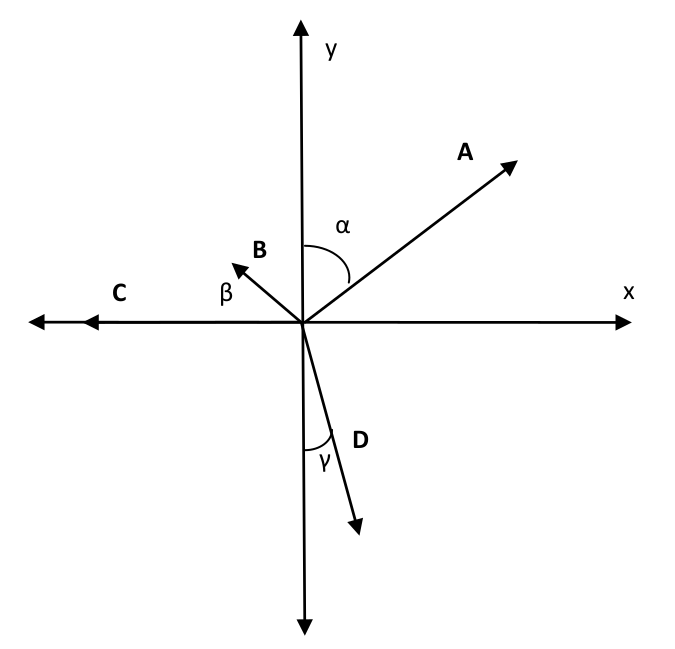
\includegraphics[clip,width = .7\columnwidth]{fig_0-7}
\end{figure}

\eje Sean los vectores como se esquematizan en la figura. Las magnitudes de cada uno son: A = 10 cm, B = 0,25 cm, C = 8 cm y D
= 9 cm. Los ángulos: α = 60\degree, β = 45\degree y γ=20\degree. 

a)Encontrar las componentes en las direcciones x e y de cada uno de ellos. 

b)Encontrar las componentes, la magnitud y la dirección respecto del eje x para el vector suma.

\eje Para los vectores \b A=(1cm, 2cm, -2cm), \b B=(-2cm, 0cm,1cm), C=(3.5cm, -1cm, 1.5cm) realizar el producto escalar de ellos con
los versores \b i, \b j, \b k. Explique el significado de realizar estos productos escalares.
\eje Encuentre el producto vectorial \b A x \b B = \b C, con \b A=(-1cm, 2cm, -2cm) y \b B=(-2cm, -0.5cm, 1cm). Verifique que \b B x \b A =- \b C


\eje Para la suma \b A+ \b B = \b C, el vector \b A tiene una magnitud de 12 m y forma un ángulo de 40°
respecto del semi-eje x positivo en sentido antihorario, y el vector \b C tiene una magnitud de 15 m
y forma un ángulo de 20° respecto del semi-eje x negativo, también medido en sentido
antihorario.

a) ¿cuál es la magnitud y el ángulo, relativo al semi-eje x positivo del vector \b B?

\eje Los vectores \b A y \b B tienen por coordenadas (en unidades arbitrarias), Ax = 3.2, Ay = 1.6, Bx
= 0.5 y By = 4.5.

a) Encuentre el ángulo entre las direcciones de ambos vectores.

b) Encuentre las coordenadas de un vector \b C que sea perpendicular a \b A, esté en el plano xy y
tenga una magnitud de 5.
\end{document}